\documentclass{ajc}
\usepackage{siunitx}
\sisetup{
	output-decimal-marker = {,},
	per-mode=fraction,
	fraction-function=\tfrac
}
\pdfsuppresswarningpagegroup=1


\title{Physik}
\author{Alexander Jacob}
\date{Schuljahr 2024/2025}

\begin{document}
	\section{Schwingungen und Wellen}
	
	\subsection{Teilaufgabe Physikabitur G-Kurs '22 HT}
	\paragraph{Kontext:}Ein Wagen der Masse $m$ ist an einer dehn- und stauchbaren Feder mit der Federkonstanten $D = \SI{50}{\newton\per\meter}$ befestigt. Für die Rückstellkraft gilt ein lineares Kraftgesetz. In Abbildung \ref{fig:wag_ggwl} befindet sich der Wagen in der Gleichgewichtslage, so dass keine Rückstellkraft wirkt. Der Wagen wird nun wie in Abbildung \ref{fig:wag_al} dargestellt um \SI{10}{\cm} aus der Gleichgewichtslage ausgelenkt und zum Zeitpunkt \SI{0}{\s} losgelassen.
	\begin{figure}[ht]
		\centering
		\begin{minipage}[b]{0.4\textwidth}
			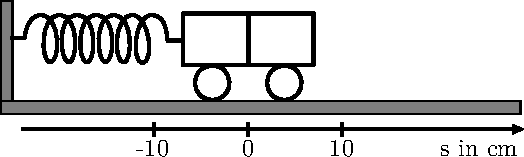
\includegraphics[width=\textwidth]{ph_wagen_ggwl.pdf}
			\caption{Wagen in Gleichgewichtslage.}
			\label{fig:wag_ggwl}
		\end{minipage}
		\hfill
		\begin{minipage}[b]{0.4\textwidth}
			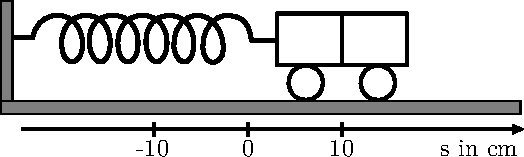
\includegraphics[width=\textwidth]{ph_wagen_al.pdf}
			\caption{Wagen in Auslenkung von \SI{10}{\cm}.}
			\label{fig:wag_al}
		\end{minipage}
	\end{figure}

	\subsubsection{Rückstellkraft berechnen}
	\paragraph{Aufgabe:}Berechnen Sie den Betrag der Rückstellkraft, die in der Abbildung \ref{fig:wag_al} dargestellten Situation wirkt, und zeichnen Sie einen Kraftpfeil ein, sodass deren Richtung erkennbar ist.
	\begin{equation}
		F_\text{rück} = \SI{50}{\newton\per\meter} \cdot \SI{0.1}{\meter} = \SI{5}{\newton}
	\end{equation}
	
	\subsubsection{Werte bestimmen}
	\paragraph{Aufgabe:}Das Diagramm in \ref{fig:wag_dia} zeigt für die Bewegung des Wagens den zeitlichen Verlauf der Elongation.
	
	Bestimmen Sie die folgenden Größen:
	\begin{itemize}
		\item die Masse $m$,
		\item den maximalen Betrag $v_\text{max}$ der Geschwindigkeit,
		\item den maximalen Betrag $a_\text{max}$ der Beschleunigung des Wagens.
	\end{itemize}
	
	\begin{figure}[ht]
		\centering
		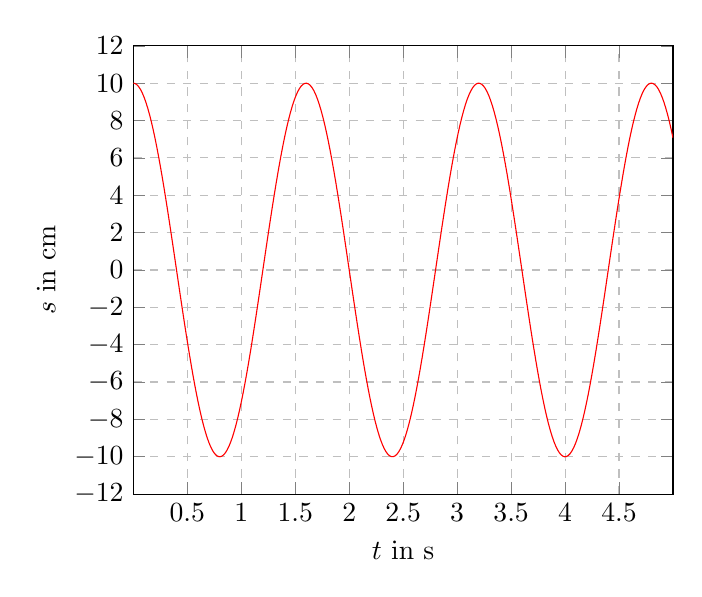
\begin{tikzpicture}
			\begin{axis}[
				xlabel={$t$ in \SI{}{\s}},
				ylabel={$s$ in \SI{}{\cm}},
				xmin=-0, xmax=5,
				ymax=12, ymin=-12,
				xtick={0.5,1.0,1.5,2.0,2.5,3.0,3.5,4.0,4.5},
				ytick={-12,-10,-8,-6,-4,-2,0,2,4,6,8,10,12},
				xmajorgrids=true,
				ymajorgrids=true,
				grid style=dashed,
				]
				\addplot [
				domain=0:5, 
				samples=300, 
				color=red,
				]
				{10 * cos(((2 * pi)/(1.6)) * deg(x))};
			\end{axis}
		\end{tikzpicture}
		\caption{Zeitlicher Verlauf der Elongation.}
		\label{fig:wag_dia}
	\end{figure}
	
	\paragraph{Masse $m$:} Aus $\omega = \frac{2\pi}{T}$ und $\omega^2 = \frac{D}{m}$ ergibt sich für die Masse $m$:
	\begin{equation}
		m = \frac{D \cdot T^2}{4\pi^2}
	\end{equation}
	
	Mit den abgelesenen Werten aus dem Diagramm \ref{fig:wag_dia} ergibt sich somit für den Betrag der Masse $m$:
	\begin{equation}
		m = \frac{\SI{50}{\newton\per\meter} \cdot (\SI{1.6}{\s})^2}{4\pi^2} = \SI{3.24}{\kg}.
	\end{equation}
	
	\paragraph{Geschwindigkeit $v_\text{max}$:} Da die Steigung des Graphen aus \ref{fig:wag_dia} z.B. zum Zeitpunkt $t = \SI{1.2}{\s}$ am größten ist, muss dort auch dessen zeitliche Ableitung $v(t)$ ein Maximum besitzen. Durch Einsetzen der Werte in das allgemeine Geschwindigkeits-Zeit-Gesetz der Federschwingung ergibt sich für den maximalen Betrag $v_\text{max}$ der Geschwindigkeit:
	\begin{equation}
		v_\text{max} = v(\SI{1.2}{\s}) = - \frac{2\pi}{\SI{1.6}{\s}} \cdot \SI{0.1}{\meter} \cdot \sin\left(\frac{2\pi}{\SI{1.6}{\s}} \cdot \SI{1.2}{\s}\right) = \SI{0.393}{\m\per\s}.
	\end{equation}
	
	\paragraph{Beschleunigung $a_\text{max}$:} Die Steigung von $v(t)$ ist zum Zeitpunkt $t = \SI{0.8}{\s}$ am größten. Daher ergibt sich für den maximalen Betrag $a_\text{max}$ der Beschleunigung des Wagens:
	\begin{equation}
		a_\text{max} = a(\SI{0.8}{\s}) = - \left(\frac{2\pi}{\SI{1.6}{\s}}\right)^2 \cdot \SI{0.1}{\meter} \cdot \cos\left(\frac{2\pi}{\SI{1.6}{\s}} \cdot \SI{0.8}{\s}\right) = \SI{1.54}{\m\per\s\squared}.
	\end{equation}
	
	\subsubsection{Zusätzliches Gewicht}
	\paragraph{Aufgabe:}In dem Moment, in dem der Wagen die maximale Elongation erreicht, wird ein Gewichtsstück aufgebracht, so dass sich die Masse des Wagens Vervierfacht. Geben Sie jeweils begründet an, ob und gegebenenfalls um welchen Faktor sich dadurch die Schwingungsdauer und der Betrag der maximalen Beschleunigung ändert.
	
	\paragraph{Schwingungsdauer:} Die Schwingungsdauer verdoppelt sich, da für $T$ gilt:
	\begin{equation}
		T = 2\pi \cdot \sqrt{\frac{m}{D}}.
	\end{equation}
	
	Wird also $m$ vervierfacht, so ändert sich $T$ um den Faktor $\sqrt{4} = 2$ und wird verdoppelt.
	
	\paragraph{Maximale Beschleunigung:} Die maximale Beschleunigung verringert sich, da $a_\text{max}$ gemäß des Beschleunigungs-Zeit-Gesetzes 
	\begin{equation}
		a(t) = -\omega^2 s_\text{max} \cdot \cos\left(\omega t\right)
	\end{equation}
	
	von $\omega^2 s_\text{max}$ abhängt. Aus der Aufgabenstellung ergibt sich, dass $s_\text{max}$ unverändert bleibt. Da $\omega^2$ gemäß $\omega^2 = \frac{D}{m}$ umgekehrt proportional zu $m$ ist, verändert sich $a_\text{max}$ um den Faktor $\frac{1}{4}$.

\end{document}